% =====================================================================
% Data section, merge-ready copy generated by Data section/build/make_final.py
% from manuscript/data-section-draft.tex (do not edit here; edit the draft and rerun).
% Sources of every number: the '% Evidence:' comments and Data section/handoff.md.
% =====================================================================
\section{How the SMOTE Literature Uses Data}
\label{sec:data}

A reader who wants to compare two SMOTE variants, or to choose a benchmark for a
new one, needs answers to questions that the papers rarely answer together.
Can the numbers that two papers report on a dataset of the same name be
compared? How broad is the evidence behind the benchmarks the field relies on?
How difficult, beyond the imbalance ratio, are the datasets that can be
checked? When a paper reports that its method beats SMOTE, on what kind of data does
that happen, and can a reader check it? This section answers these questions
from the 1,747 dataset entries and the comparisons with SMOTE that we extracted from the
76 papers of our corpus: 835 under one fixed metric per paper (834 per dataset and one
average over datasets) and 2,497 over every metric the papers report. Three of them (ENN, AdaBoost and one review) contain no
evaluation on data, so counts below use the 73 papers with an
evaluation on data; Tomek links is kept because it illustrates its method on
one synthetic two-class set.

The central observation is that the evidence for a new oversampler is only as
interpretable as the description of its data, and in this literature that
description is often incomplete: the same name can denote different tasks, many
modifications are not described well enough to be repeated, and 14 of the 57 papers
that use SMOTE as a baseline give no per-dataset pair of scores against it. Where
per-dataset results exist, the proposed method beats plain SMOTE in about four of five
decided comparisons. These wins are not more frequent on data the authors modified,
but they are more frequent on data whose minority examples are borderline or isolated,
and they are much less consistent on precision and specificity than on the other metrics.

% ---------------------------------------------------------------------
\subsection{Extraction Procedure}
\label{sec:data-method}
For every paper we read the full text and any supplementary file in our
collection, and recorded each dataset as printed, including spelling, with
its group in the paper, source repository, size, number of features and
classes, minority and majority counts, and the imbalance ratio where the
paper prints them, together with the table and page they come from. For each
dataset we also recorded how it reached the experiment:
\emph{original} (used as distributed, with its native classes),
\emph{repository-defined} (a two-class split published by a repository such
as KEEL or imbalanced-learn, used as is), \emph{modified} (the authors chose
the minority classes, merged or dropped classes, set a threshold, undersampled
or injected noise), or \emph{synthetic} (generated by the authors). Where a
paper did not state its source, two fixed rules were applied and flagged:
names that follow the KEEL file convention (for example
\texttt{ecoli-0-1\_vs\_5}, \texttt{yeast4}) were labelled repository-defined,
and common names in multiclass papers with no stated change were labelled
original. Two further rules were fixed before counting: a set that is two-class
in its source and is used without comment was labelled original, and a set from
which the authors removed rows (for example, records with missing values) or
attributes was labelled modified. A set whose source the paper does not state, for which it
prints no size, and whose name identifies a public unmodified file was labelled original (four
entries). One label rests on evidence outside the paper: the \texttt{toy} set of
OREM-M, listed without a source, is the synthetic set of the ordinal-regression
benchmark~\parencite{gutierrez2016ordinal} and is labelled synthetic.

For the results we copied, per dataset, the printed score of the proposed
method and of SMOTE from one results table selected by a fixed rule:
G-mean, else AUC, else F-measure, else accuracy; the classifier highlighted
in the abstract, else the first reported; the unperturbed condition. We
recorded values rather than wins so that any definition of a win can be
applied later. From the same table setting we then copied every other metric that the
paper reports for both methods (2,497 dataset-by-metric values in 44 papers); the
fixed-metric values were copied a second time in this pass, independently, and agree
on all 839 rows that both copies contain. Plain SMOTE was distinguished from SMOTE embedded in a
multiclass or ensemble wrapper (Static-SMOTE, OVO-SMOTE~\parencite{fernandez2013analysing}, SMOTE-all,
SMOTE+AdaBoost). Values printed in a paper are never overwritten; corrections
against the source repository are stored beside them with their justification.
Every extracted value was then checked against the PDF a second time: a value
was accepted when the dataset name and its numbers appear on the same line of
the cited page, and every table that is printed as an image or whose text layer
is garbled was read from the rendered page instead. All 1,654 dataset entries
of the first extraction and 835 fixed-metric comparisons passed this check (the 93 sets added on 8 November were checked the same way, with a quoted sentence on the cited page); the values of the other metrics
were read once, from the text layer or the rendered page.

% Evidence: ai-draft/full/SCHEMA.md; build/full\_extraction.py; KEEL and
% multiclass rules approved by Toon 18 Oct, rules A and B 18 Oct; 454 extraction notes in
% out/full\_uncertain.csv, each resolved in out/uncertain\_resolution.csv; second check:
% build/verify\_pdf.py, out/visual\_checks.json, out/verified\_*.csv; values also checked by Toon against the PDFs
% (28 Oct 2026).

% Toon 28 Oct 2026: state only that the values were checked; no blind agreement rate is reported.

% ---------------------------------------------------------------------
\subsection{The Benchmark Landscape}
\label{sec:data-landscape}
The 73 papers with an evaluation on data list 1,747 dataset entries, counting the
93 sets that ten papers generate only for an illustration or a side experiment
(Section~\ref{sec:data-verifiability}). One of them, the single toy example in Tomek links, is a description rather than a
name and is set aside here, leaving 1,746 named entries. These reduce to 857
distinct names once names are lower-cased, text in parentheses is dropped, and
underscores and spaces are treated alike. Treating spellings that differ only in
punctuation as one dataset (\texttt{page-blocks}, \texttt{pageblocks} and the singular
\texttt{page-block}) leaves 766 datasets, and grouping each numbered or split version with its main set (for
example \texttt{yeast4} or \texttt{glass-0-1-6\_vs\_2} with yeast and glass),
while keeping non-standard names such as \texttt{glass identification} apart,
leaves 482 source families. Most datasets appear once: 543 of the 766 occur in a
single paper (60 of them are the generated sets of a single experiment in MC-MBRC~\parencite{ma2024mcmbrc}, which form one family). Counted as datasets, ecoli appears in 29 papers, yeast in 22 and
glass in 19; counted with their splits, the ecoli family appears in 42 papers,
the yeast family in 39 and the glass family in 35, about half of the 73. Half of
all uses of a family fall on 40 of the 482 families. Names whose printed number of
features contradicts their main set are kept in its family when they are the same
source with a different composition (for example \texttt{abalone8}, \texttt{oil1}) and
kept apart when they are a different data set that shares the prefix (for example
\texttt{car1}, a microarray set with 9,182 features).

Splits cut from one source are not copies of each other. Among the verifiable
two-class KEEL files (Section~\ref{sec:data-difficulty}), the 14 yeast splits
range in imbalance ratio from 2.5 to 41.4 and in noise index from 0.29 to 0.86,
and the 19 ecoli and 13 glass splits from 0.12 to 0.69 and from 0.24 to 0.77.
They do share the source's attributes (7 or 8 for yeast, 6 or 7 for ecoli, 9 for
glass), its domain and often its examples: \texttt{yeast4} and
\texttt{yeast-0-5-6-7-9\_vs\_4} use the same 51 minority examples and differ
only in which classes form the majority.

Outcomes on splits of one source are also related. In the eleven papers that
compare with plain SMOTE on several splits of the same source (282 per-dataset
comparisons, 262 same-family pairs; families by the rule in the evidence note),
whether the proposed method wins does not cluster by family (pairs agree on win,
tie or loss in 0.60 of cases, as under random relabelling), but the size of its
margin does: the within-paper ranks of the margin differ by 0.29 on average for
two splits of one source against 0.34 when family labels are permuted within each
paper ($p = 0.005$, 10,000 permutations; leaving out one paper at a time gives
$p$ between 0.002 and 0.048).

% Toon's own wording (28 Oct 2026), not a Claude draft.
Splits cut from one source vary the task (its imbalance ratio and where the
minority examples lie) but not the source (its domain, attributes and
dimensionality), and within the papers that evaluate several splits of one
source, the margin over SMOTE tends to be slightly more alike within a family
than between families. Papers should therefore report the number of source
families alongside the number of datasets, and should not treat each split as
independent evidence.

\paragraph{What the reader should do.} %
Report the source family
of each dataset alongside the count, so that readers can see how many
independent sources stand behind a claim, and keep splits of one source
together when testing for significance.

% Evidence: out/verified\_datasets.csv; counts reproduced by build/reconcile\_counts.py
% (out/reconcile\_counts.json): rule R1 sets aside the Tomek links placeholder (row 1558,
% kept in the file), R2 normalises with build/analyse\_dataset\_usage.py norm(), R3 gives
% exact-name, dataset and family counts under rule T1 (build/family\_rule.py, out/dataset\_families.csv; the earlier prefix
% count gave 39/39/36 and is superseded); datasets and families per name: out/landscape\_families.csv; concentration by
% dataset and family: out/benchmark\_concentration.json. With the placeholder the counts are 858 and 627;
% removing all punctuation would leave 678 names. The 605 names of the 6 Oct list are
% superseded by the 771 of the full re-read (857 after the 93 generated sets of build/add\_synthetic\_entries.py, 8 Nov 2026). Spread within the yeast, ecoli and glass
% families: difficulty/family\_spread.py $\rightarrow$ family\_spread.json. Datasets and families
% everywhere in this subsection: rule T1 (Toon, 28 Oct 2026; names differing only by punctuation are one dataset, numbered
% or split versions belong to their main set, non-standard names are not merged), build/family\_rule.py
% $\rightarrow$ out/dataset\_families.csv; outcomes linked to records through out/outcome\_dataset\_links.csv;
% build/family\_dependence.py $\rightarrow$ out/family\_dependence.json (key t1).

% Dataset landscape for cross-family comparison (added 19 Oct 2026 from
% manuscript/proposal_dataset_landscape.tex, reviewed against out/ files).
% Group labels F/D/V approved by Toon 28 Oct 2026 (approval slot removed).
\paragraph{Candidate benchmarks for a cross-family comparison.}
Table~\ref{tab:data-candidates} lists 18 datasets considered as benchmarks for
comparing method families: the 11 datasets we set out to
examine and the datasets that meet one of two written rules. The first rule
takes every dataset used by at least ten papers (33 datasets). The second takes
datasets used by three to nine papers whose every printed size is at least 10,000
instances, a size that no entry of the first group reaches (7 datasets). The
groups follow from these two rules on use and printed
size only and say nothing about overlap, noise, sparsity, feature type or any
other property. IR is not used, because its definition differs between papers.
No dataset used by three or more papers is printed with 100 or more features
every time it is reported; this is a property of the rule, not evidence that
the corpus contains no high-dimensional data sets.

Family counts follow the same rule for every dataset. The dataset \texttt{shuttle} is printed with four different
sizes (2,175, 14,500, 43,500 and 57,999 instances) and once without a size.
Two pairs of papers print matching sizes and class counts; the other versions
are single reports, and OVO-SMOTE prints five classes in one table and seven
class counts in another. The versions are therefore kept apart and not pooled.

The frequently used benchmarks are small: among the entries that
print a size, half have 800 or fewer instances and half have nine or fewer
features. Names printed with 10,000 or more instances in every paper are used
by three to nine papers each, so a comparison across method families that
wants to cover data size has to look beyond the frequent set.

\begin{table}[t]
\centering\small
\caption{Data Sets Considered as Benchmarks for Cross-Family Comparison.
F: used by ten or more papers; D: used by three to nine
papers, every printed size at least 10,000 instances; V: needs verification.
Papers count the dataset (spellings that differ only in punctuation are one
dataset); family papers include the numbered and split versions of the dataset.
Values are as printed and differ between papers. $^{a}$Four printed versions, not pooled.}
\label{tab:data-candidates}
\begin{tabular}{@{}llrrrrlr@{}}
\toprule
Dataset & Group & Papers & Family papers & Instances & Size printed & Classes & Modified\\
\midrule
% >>> landscape-candidates rows (generated by build/landscape_manuscript.py; do not edit by hand)
\texttt{ecoli} & F & 29 & 42 & 301--336 & 25/31 & 2, 4, 5, 8 & 8/31\\
\texttt{page-blocks} & F & 22 & 34 & 545--5,476 & 17/22 & 2, 4, 5 & 6/22\\
\texttt{yeast} & F & 22 & 39 & 483--1,485 & 16/22 & 2, 6, 8, 9, 10 & 4/22\\
\texttt{pima} & F & 21 & 21 & 590--769 & 19/23 & 2 & 2/23\\
\texttt{vehicle} & F & 21 & 30 & 713--940 & 19/23 & 2, 3, 4 & 10/23\\
\texttt{haberman} & F & 20 & 20 & 252--306 & 19/22 & 2 & 2/22\\
\texttt{glass} & F & 19 & 35 & 167--214 & 18/21 & 2, 6 & 7/21\\
\texttt{balance} & F & 16 & 16 & 625 & 14/16 & 3 & 3/16\\
\texttt{wine} & F & 16 & 16 & 130--178 & 15/18 & 2, 3 & 6/18\\
\texttt{satimage} & F & 15 & 16 & 6,430--6,435 & 11/15 & 2, 6, 7 & 8/15\\
\texttt{letter} & D & 9 & 9 & 11,057--20,000 & 9/9 & 2, 26 & 6/9\\
\texttt{nursery} & D & 7 & 7 & 12,690--12,960 & 7/7 & 2, 4, 5 & 3/7\\
\texttt{mammography} & D & 5 & 5 & 11,183 & 4/5 & 2 & 0/5\\
\texttt{adult} & D & 3 & 3 & 32,562--48,842 & 2/3 & 2 & 1/3\\
\texttt{avila} & D & 3 & 4 & 10,430--20,850 & 3/3 & 2, 11 & 1/3\\
\texttt{default} & D & 3 & 3 & 30,000 & 2/3 & 2 & 0/3\\
\texttt{shoppers} & D & 3 & 3 & 12,330--12,331 & 3/3 & 2 & 0/3\\
\texttt{shuttle} & V & 7 & 15 & 2,175--57,999$^{a}$ & 6/7 & 2, 5 & 1/7\\
% <<< landscape-candidates rows
\bottomrule
\end{tabular}
\end{table}

% Groups F, D and V approved by Toon 28 Oct 2026 (family rule T1, 28 Oct 2026).

\paragraph{Limits of the evidence.}
Size, dimensionality and the number of classes are printed for 75.9\%, 72.7\%
and 78.4\% of the 1,746 named entries, and class proportions in some form for
54.8\%. A measured class overlap exists for 36 entries in two papers, on two
incompatible scales, and the curated evidence contains no statement about
sparsity. %
What the papers print therefore cannot show which ranges of
overlap, noise or sparsity the benchmarks cover; the candidates in
Table~\ref{tab:data-candidates} are chosen on use and size only.
Section~\ref{sec:data-difficulty} measures these properties directly for the
entries whose files can be identified.

% Evidence: out/benchmark\_candidates.csv and .json (build/landscape\_candidates.py;
% rules and approval status in \texttt{criteria}); table rows written by
% build/landscape\_manuscript.py; out/landscape\_families.csv (446 groups, 82
% flagged and left unmerged); out/shuttle\_versions.csv (build/shuttle\_versions.py;
% OVO-SMOTE Table 2 and Table 3, p.6, checked 19 Oct); out/characteristics\_coverage.json;
% out/benchmark\_concentration.json. All records are browsable in the Atlas
% (manuscript tab and Landscape tab).

% ---------------------------------------------------------------------
\subsection{How Datasets Are Chosen and Modified}
\label{sec:data-handling}

\begin{table}[t]
\centering\small
\caption{How the Papers Choose and Obtain Their Data.
Top: paper level, 73 papers with an evaluation on data. Bottom: dataset entries.}
\label{tab:data-handling}
\begin{tabular}{lr}
\toprule
Item & Count\\
\midrule
\multicolumn{2}{l}{\emph{Reason given for the choice of datasets (papers)}}\\
\quad Own reason (diversity, difficulty, application, \ldots) & 48\\
\quad Cites prior work & 14\\
\quad ``Widely used'' only & 3\\
\quad Not stated & 8\\
Benchmark list adopted from earlier work, declared (papers) & 20 (wholesale 11)\\
Binarised, minority rule not stated (papers) & 8 of 37\\
\addlinespace
\multicolumn{2}{l}{\emph{How each dataset entry reached the experiment}}\\
\quad Original & 537\\
\quad Repository-defined (KEEL, imbalanced-learn) & 470\\
\quad Modified by the authors & 332\\
\quad Synthetic & 213\\
\quad Cannot be told from the paper & 195\\
\bottomrule
\end{tabular}
\end{table}

Table~\ref{tab:data-handling} shows that modification by the authors is
common: 332 of 1,747 dataset entries were changed by the
authors themselves, and for 195 the paper does not let a reader
tell how the data were obtained. Eleven papers give no reason for their
choice of datasets or only call them widely used.

Modification is not a fault in itself: binarising a multiclass
set or raising the imbalance ratio are legitimate ways to probe a method.
What matters for the reader is whether the modification is declared where a
reader looks for it. A KEEL file name such as \texttt{yeast-0-5-6-7-9\_vs\_4}
declares its split; a paper that prints only ``Yeast'' after choosing its own
minority classes does not.

Modifications differ in how completely they are described. Of the 332 modified
entries (39 papers), 177 in 30 papers change the class structure, most often by
keeping one class against the rest (84 entries), and 147 in 9 papers raise the
imbalance ratio on purpose, almost always by removing minority examples at random
(131 entries). A purpose for the change is stated in 15 of the 39 papers. For 94 of
the 332 entries, information needed to repeat the change is missing: the
characteristics of the modified set are not printed for 56, the target imbalance
ratio for 18 and the minority class for 15. At the paper level, 8 of the 37 papers
that binarise data do not state which class becomes the minority. Entries modified
without printed characteristics cannot be matched to any public file unless the authors
publish the modified data themselves, as k-means SMOTE does; 48 such entries
are therefore left out of the difficulty measurement (Section~\ref{sec:data-difficulty}).

% Evidence: out/data\_handling\_summary.json (paper-level codes; binarised\_without\_stated\_rule,
% minority\_rule\_among\_binarised); out/full\_summary.json how\_obtained\_all (entry level, with rules);
% operations, purposes and missing information: build/modified\_operations.py $\rightarrow$
% out/modified\_operations\_audit.csv and out/modified\_operations\_summary.json (Analysis A).

% ---------------------------------------------------------------------
\subsection{The Same Name Is Not the Same Data}
\label{sec:data-names}
Of the 192 datasets that at least two papers print with a size (spellings that
differ only in punctuation counted as one dataset), 90 appear with more than one size: thyroid with 7,200 instances in five papers and
720 in four, dermatology with 358 (the KEEL version) in eight and 366 (UCI) in
two, ecoli with 336, 327, 310 and 301, and pima with 768, 769, 635 and 590.
Some of these differences are declared subsamples; the name alone does not tell
which. MWMOTE~\parencite{barua2014mwmote} illustrates the problem inside a single paper:
its Satimage (6,435 instances) and Statlandsat (4,435) are the full Statlog
Landsat set and its training file, counted as two of its twenty datasets,
and its common names are ambiguous in both directions (its Ecoli matches the
KEEL file \texttt{ecoli1} exactly, while its Yeast matches no published split).

Imbalance ratios add a second layer. Table~\ref{tab:ir-definitions} lists the
definitions found in the corpus; some are not convertible into one another,
and some papers print IR without a formula.

\begin{table}[t]
\centering\small
\caption{Imbalance-Ratio Definitions Printed in the Papers}
\label{tab:ir-definitions}
\begin{tabular}{p{0.28\linewidth}p{0.3\linewidth}p{0.32\linewidth}}
\toprule
Definition & Formula & Used by (examples)\\
\midrule
Largest over smallest class & $N_{\max}/N_{\min}$ & MDO~\parencite{abdi2016mdo}, CBHSID~\parencite{palli2022cbhsid}, MKC-SMOTE~\parencite{wang2024mkc} (its $IR$)\\
Majority over minority (binary wording) & $N_{\mathrm{maj}}/N_{\mathrm{min}}$ & OVO-SMOTE (defined for the binary case, applied to multiclass sets)\\
Percentage minority & $100\,N_{\min}/N$ & RUSBoost~\parencite{seiffert2010rusboost}\\
Per-class imbalance degree & $\sum_{q\neq i} N_q/((C-1)N_i)$ & OREM-M~\parencite{zhu2023orem} (overall IR only cited, not printed)\\
Summed pairwise multiclass IR & $\sum_{i<j} (N_i/N_j - 1)$ & SMOM~\parencite{zhu2017smom}, GDHS~\parencite{yan2025gdhs}, MKC-SMOTE ($IR_{\mathrm{overall}}$)\\
Imbalance degree $Id$ & distance from uniform \parencite{ortigosahernandez2017imbalance} & SHSampler~\parencite{zheng2022shsampler} (cited, no formula printed)\\
Minimum class prior & $N_{\min}/N$ & DSRBF~\parencite{fernandeznavarro2011dsrbf}\\
Coefficient of variation & $\mathrm{sd}(N_i)/\mathrm{mean}(N_i)$ & COG-OS~\parencite{wu2007cogos}\\
Proportion pair & e.g.\ $0.04{:}0.96$ & MWMOTE (wording: minority to majority)\\
Not stated (values equal $N_{\max}/N_{\min}$) & n/a & MC-CCR~\parencite{koziarski2020mcccr}, MC-RBO~\parencite{krawczyk2020mcrbo}\\
\bottomrule
\end{tabular}
\end{table}

Errors also travel with shared benchmark tables: MC-CCR and
MC-RBO both print an IR of 1.17 for vehicle, a value no definition produces
from its class counts.

\paragraph{What the reader should do.} %
Compare results across
papers only after mapping each name to its exact file and class split, and
report the IR formula together with its values.

% Evidence: out/verified\_datasets.csv: names normalised, printed n\_instances compared across
% papers (192 datasets, rule T1, with a printed size in two or more papers; 198 if spellings are kept apart;
% out/reconcile\_counts.json size\_variation); the earlier 20 of 75 from
% ai-draft/dataset\_variants.json covered 8 papers only and is superseded;
% mwmote-table5-audit.md; extraction-notes.md; full re-read ir\_definition per
% paper in out/full\_summary.json.

% ---------------------------------------------------------------------
\subsection{How Difficult Are the Datasets That Can Be Checked?}
\label{sec:data-difficulty}
% Revised 8 Nov 2026 (Claude; Toon asked to measure every dataset that can be obtained): second
% verification pass over extended mirrors (difficulty/verify_ext.py), 643 -> 864 verifiable entries,
% 113 -> 151 two-class tasks; second round the same day (official UCI and LibSVM files, authors'
% repositories, Part-B entries): 973 verifiable entries, 227 two-class tasks; third round (Kaggle, header-row rule
% for Loyalty-SMOTE, rule NS): 986 entries, 236 tasks.
% Numbers: difficulty/profile_final_summary.json, verify_ext_summary.json.
The papers rarely describe how hard their data are beyond the imbalance ratio.
A numerical overlap measure is printed for 36 of the 1,746 named entries, all in
two papers, and noise or borderline examples are described for 5; three of 72
papers report such a property of their original data
(Section~\ref{sec:data-landscape}). The literature on imbalanced learning, however,
attributes much of the difficulty of these problems to characteristics of the data other
than the imbalance ratio: overlap between the classes, noisy and borderline examples,
small disjuncts and a shortage of minority examples
\parencite{jo2004smalldisjuncts,lopez2013insight,napierala2016types}.
We therefore measured these characteristics ourselves on the entries whose data can be
identified. An entry counts as verifiable when its name matches a public file and the
printed number of instances (and of minority examples, when printed) equals that file's,
or when the paper prints no size, the name matches a public file and the authors did not
modify the data, or when the authors publish the modified file themselves under the
entry's name (k-means SMOTE~\parencite{douzas2018kmeans}). One paper (Loyalty-SMOTE) prints, for eight
entries, a size exactly one larger than the public file, apparently counting the header line; for
this paper a printed size of the file's size plus one is accepted. A two-class file is not accepted
for an entry whose paper prints more than two classes. The files come from KEEL \parencite{alcalafdez2011keel}, the UCI repository
\parencite{kellyucirepository} (downloaded from the repository, and through the UCI++ collection \parencite{garciaucipp}, the UCI files
distributed with Weka and single-file copies), LIBSVM \parencite{chang2011libsvm}, PMLB \parencite{romano2022pmlb}, imbalanced-learn
\parencite{lemaitre2017imbalanced}, the PROMISE defect data \parencite{jureczko2010towards} and the
repositories in which five papers publish their own processed data, and Kaggle for the sets that
papers take from it. A name is
looked up under the other published names of the same data set (liver disorders is
\texttt{bupa}, contraceptive method choice is \texttt{cmc}), but only the printed size decides
whether a file is accepted. This holds for 986 entries from 65 papers, which use 256 files.
Entries modified by their authors without printed characteristics and without a published
file (48) are left out, because the data actually used cannot be reconstructed.

Each two-class file, each binarisation that a paper describes precisely enough to reproduce,
and each imbalanced-learn task defines one task: 236 tasks, used by 701 entries in 46 papers.
One-vs-rest tasks that we built from multiclass files (339) are not tasks any paper
evaluated and are reported apart. Every minority example is labelled safe,
borderline, rare or outlier from the classes of its five nearest neighbours
\parencite{napierala2016types}, with distances measured by HVDM
\parencite{wilson1997improved}. The noise index of a task is the share of minority examples
that are borderline or outliers; we report it as a continuous value because we found no
published threshold for it. Three flags use published thresholds: small disjuncts when at
least 20\% of minority examples are rare and outliers when more than 20\% are
outliers \parencite{napierala2016types}, and small sample when there are fewer than ten
minority examples per feature \parencite{jain2000statistical}. The imbalance ratio
$N_{\mathrm{maj}}/N_{\mathrm{min}}$, computed from the files, is grouped into the
bands 1.5 to 3, 3 to 9 and above 9 \parencite{fernandez2008study} and is not used as a
difficulty flag.

\begin{table}[t]
\centering\small
\caption{Difficulty Profile of the Verifiable Tasks. A task can carry several flags;
entries count how often the corpus uses a task.}
\label{tab:data-difficulty}
\begin{tabular}{lrrr}
\toprule
 & \multicolumn{2}{c}{Binary and binarised} & One-vs-rest\\
 & Tasks & Entries & Tasks\\
\midrule
All & 236 & 701 & 339\\
Small disjuncts (rare $\geq$ 20\%) & 33 (14\%) & 65 (9\%) & 26 (8\%)\\
Outliers ($>$ 20\%) & 83 (35\%) & 198 (28\%) & 43 (13\%)\\
Small sample ($N_{\min}/d < 10$) & 160 (68\%) & 454 (65\%) & 157 (46\%)\\
None of the three & 63 (27\%) & 222 (32\%) & 172 (51\%)\\
Imbalance ratio $>$ 9 & 139 & 375 & 157\\
Noise index, median [P25, P75] & \multicolumn{2}{c}{0.58 [0.29, 0.77]} & 0.28 [0.07, 0.61]\\
\bottomrule
\end{tabular}
\end{table}

Table~\ref{tab:data-difficulty} shows that the most common property of the binary
tasks is a small sample: 160 of 236 have fewer than ten minority examples per
feature. The flags combine in seven profiles: small sample alone (87 tasks), small sample
with outliers (42), all three flags (28), outliers alone (11), small disjuncts with a small
sample (3), small disjuncts with outliers (2) and none (63). The noise index separates tasks that the flags do not
(Figure~\ref{fig:data-difficulty}a): among the 63 tasks without a flag it ranges from 0 to
0.84, with 20 tasks at 0.5 or above (haberman 0.84, the numeric German credit data 0.81,
contraceptive 0.79 and bupa 0.79 among them) and 16 below 0.1. Its median is 0.31, 0.44,
0.48 and 0.66 in the imbalance-ratio bands up to 1.5 (6 tasks), 1.5 to 3 (40), 3 to 9 (51)
and above 9 (139), and its rank correlation with the imbalance ratio is 0.26.

\begin{figure}[t]
\centering
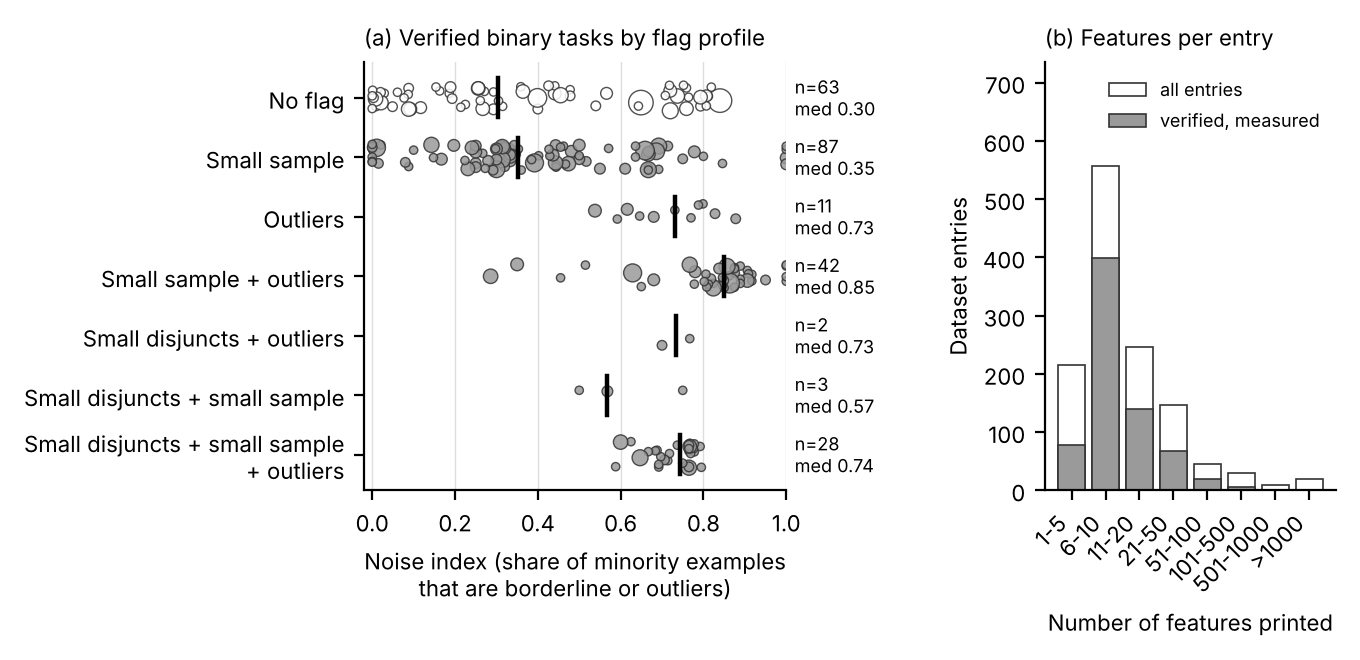
\includegraphics[width=\linewidth]{figures/data-difficulty}
\Description{Left: dot plot of the noise index (0 to 1) for 236 binary tasks in seven rows by flag profile, with medians 0.30 (no flag, 63 tasks), 0.35 (small sample, 87), 0.73 (outliers, 11), 0.85 (small sample and outliers, 42), 0.73 (small disjuncts and outliers, 2), 0.57 (small disjuncts and small sample, 3) and 0.74 (all three flags, 28). Right: bar chart of dataset entries by printed number of features; most entries have 6 to 10 features and only six entries above 100 features could be verified.}
\caption{(a) Noise index of the 236 verifiable binary and binarised tasks, one row
per flag profile; marker area grows with the number of entries that use the task,
and the vertical bar marks the median. (b) Number of features printed for the
1,271 entries that report it, with the entries that could be verified and measured.
The bins are for display only.}
\label{fig:data-difficulty}
\end{figure}

The measurable part of the corpus is also low-dimensional
(Figure~\ref{fig:data-difficulty}b). The printed number of features has a median
of 9 and half of the entries lie between 4 and 10 features. The 59 entries with more
than 100 features come from 54 names in 18 papers, no name is used by more than two
papers, and only six of them could be verified (musk twice, isolet, and madelon, a1a and mushrooms in the
files that HDE publishes); the verified tasks have at most 617 features (median 9).

The imbalance ratio, the one difficulty-related number most papers
print, says little about where the minority examples lie: tasks with a low ratio
can be as mixed as tasks with a high one, and a task without any flag is not
necessarily easy. Conclusions drawn from the common benchmarks speak mainly for
small, low-dimensional tables with few minority examples per feature.

Most papers mix these profiles. Of the 39 papers with at least three verifiable tasks,
36 include both flagged and flag-free tasks, two (COG-OS~\parencite{wu2007cogos} and
SMOTE-ENN) use only flag-free tasks and one (GOIO) only flagged ones.
Section~\ref{sec:data-wins} relates the measured profiles to the reported wins.

\paragraph{A reference collection.} For readers who need a small benchmark that covers
the measured range, Table~\ref{tab:data-reference} selects 42 of the 236 tasks by a
fixed rule with no threshold of our own. Each combination of flag profile and
imbalance-ratio band that occurs (19 combinations) contributes the task that the
corpus uses most, for comparability with earlier results, and the tasks with the
lowest and the highest noise index, for spread. The collection spans noise indices from
0 to 1, imbalance ratios from 1.1 to 970.6 and sizes from 79 to 62,630 instances, and 13
of its files match the official KEEL table. Its tasks are not independent of one
another: it holds four yeast splits, three pima versions and two each of ecoli, glass, haberman,
cleveland, heart and iris, which should be grouped by source when results are tested.

% Table generated by difficulty/reference_collection.py (do not edit by hand); in data-section-draft.tex since 29 Oct 2026.
\begin{table}[t]\centering\small
\caption{A Reference Collection of Verifiable Two-Class Tasks. One row per selected task; Role: core = most used task in its cell, low/high = lowest/highest noise index in its cell. Profile: S small sample, O outliers, D small disjuncts; Noise: noise index; Entries: corpus entries that use the task.}
\label{tab:data-reference}
\begin{tabular}{@{}p{0.27\linewidth}lllrrrrrr@{}}
\toprule
Task & Role & Profile & IR band & $N$ & $N_{\min}$ & $d$ & IR & Noise & Entries\\
\midrule
\raggedright\texttt{banknote-\allowbreak{}authentication} & low & none & $\leq$1.5 & 1,372 & 610 & 4 & 1.2 & 0.00 & 1\\
\raggedright\texttt{bupa} & core+high & none & $\leq$1.5 & 345 & 145 & 6 & 1.4 & 0.79 & 6\\
\raggedright\texttt{smoke detection} & low & none & 1.5--3 & 62,630 & 17,873 & 14 & 2.5 & 0.00 & 1\\
\raggedright\texttt{pima} & core & none & 1.5--3 & 768 & 268 & 8 & 1.9 & 0.65 & 24\\
\raggedright\texttt{haberman} & high & none & 1.5--3 & 306 & 81 & 3 & 2.8 & 0.84 & 22\\
\raggedright\texttt{segment0} & low & none & 3--9 & 2,308 & 329 & 19 & 6.0 & 0.02 & 7\\
\raggedright\texttt{yeast3} & core & none & 3--9 & 1,484 & 163 & 8 & 8.1 & 0.40 & 13\\
\raggedright\texttt{contraceptive [minority: 2]} & high & none & 3--9 & 1,473 & 333 & 9 & 3.4 & 0.79 & 2\\
\raggedright\texttt{kr-\allowbreak{}vs-\allowbreak{}k-\allowbreak{}one\_\allowbreak{}vs\_\allowbreak{}fifteen} & low & none & $>$9 & 2,244 & 78 & 6 & 27.8 & 0.00 & 1\\
\raggedright\texttt{shuttle-\allowbreak{}c0-\allowbreak{}vs-\allowbreak{}c4} & core & none & $>$9 & 1,829 & 123 & 9 & 13.9 & 0.01 & 7\\
\raggedright\texttt{yeast-\allowbreak{}0-\allowbreak{}2-\allowbreak{}5-\allowbreak{}6\_\allowbreak{}vs\_\allowbreak{}3-\allowbreak{}7-\allowbreak{}8-\allowbreak{}9} & high & none & $>$9 & 1,004 & 99 & 8 & 9.1 & 0.57 & 4\\
\raggedright\texttt{heart} & core+low & S & $\leq$1.5 & 270 & 120 & 13 & 1.2 & 0.33 & 4\\
\raggedright\texttt{sonar} & high & S & $\leq$1.5 & 208 & 97 & 60 & 1.1 & 0.40 & 1\\
\raggedright\texttt{wine [minority: 1]} & low & S & 1.5--3 & 178 & 59 & 13 & 2.0 & 0.00 & 1\\
\raggedright\texttt{glass0} & core & S & 1.5--3 & 214 & 70 & 9 & 2.1 & 0.44 & 7\\
\raggedright\texttt{planning-\allowbreak{}relax} & high & S & 1.5--3 & 182 & 52 & 12 & 2.5 & 0.85 & 1\\
\raggedright\texttt{musk} & low & S & 3--9 & 6,598 & 1,017 & 167 & 5.5 & 0.01 & 2\\
\raggedright\texttt{ecoli3} & core & S & 3--9 & 336 & 35 & 7 & 8.6 & 0.69 & 10\\
\raggedright\texttt{hepatitis (PMLB, N=155)} & high & S & 3--9 & 155 & 32 & 19 & 3.8 & 0.75 & 2\\
\raggedright\texttt{dermatology-\allowbreak{}6} & low & S & $>$9 & 358 & 20 & 34 & 16.9 & 0.00 & 2\\
\raggedright\texttt{yeast5} & core & S & $>$9 & 1,484 & 44 & 8 & 32.7 & 0.66 & 13\\
\raggedright\texttt{cleveland-\allowbreak{}0\_\allowbreak{}vs\_\allowbreak{}4} & high & S & $>$9 & 177 & 13 & 13 & 12.6 & 1.00 & 4\\
\raggedright\texttt{shoppers} & core+low & O & 3--9 & 12,330 & 1,908 & 17 & 5.5 & 0.62 & 4\\
\raggedright\texttt{pima2} & high & O & 3--9 & 634 & 134 & 8 & 3.7 & 0.80 & 1\\
\raggedright\texttt{mammography} & core+low & O & $>$9 & 11,183 & 260 & 6 & 42.0 & 0.54 & 5\\
\raggedright\texttt{balance [minority: B]} & high & O & $>$9 & 625 & 49 & 4 & 11.8 & 0.88 & 2\\
\raggedright\texttt{heart6} & low & S+O & 3--9 & 170 & 20 & 13 & 7.5 & 0.65 & 1\\
\raggedright\texttt{breast\_\allowbreak{}tissue4} & core+high & S+O & 3--9 & 79 & 9 & 9 & 7.8 & 0.89 & 1\\
\raggedright\texttt{ecoli-\allowbreak{}0-\allowbreak{}1-\allowbreak{}3-\allowbreak{}7\_\allowbreak{}vs\_\allowbreak{}2-\allowbreak{}6} & low & S+O & $>$9 & 281 & 7 & 7 & 39.1 & 0.29 & 7\\
\raggedright\texttt{yeast4} & core & S+O & $>$9 & 1,484 & 51 & 8 & 28.1 & 0.86 & 15\\
\raggedright\texttt{ijcnn1} & high & S+O & $>$9 & 4,858 & 5 & 22 & 970.6 & 1.00 & 1\\
\raggedright\texttt{haberman2} & core+low+high & D+O & 3--9 & 265 & 40 & 3 & 5.6 & 0.70 & 2\\
\raggedright\texttt{promotion} & core+low+high & D+O & $>$9 & 23,815 & 1,634 & 4 & 13.6 & 0.77 & 1\\
\raggedright\texttt{breast.cancer} & core+low+high & D+S & 1.5--3 & 277 & 81 & 9 & 2.4 & 0.57 & 3\\
\raggedright\texttt{iris4} & core+low+high & D+S & 3--9 & 112 & 12 & 4 & 8.3 & 0.75 & 1\\
\raggedright\texttt{iris6} & core+low+high & D+S & $>$9 & 108 & 8 & 4 & 12.5 & 0.50 & 1\\
\raggedright\texttt{heart-\allowbreak{}disease-\allowbreak{}processed-\allowbreak{}cleveland [minority: 4]} & low & D+S+O & 3--9 & 303 & 35 & 13 & 7.7 & 0.71 & 1\\
\raggedright\texttt{fertility-\allowbreak{}diagnosis} & core & D+S+O & 3--9 & 100 & 12 & 9 & 7.3 & 0.75 & 1\\
\raggedright\texttt{liver\_\allowbreak{}disorders6} & high & D+S+O & 3--9 & 224 & 24 & 6 & 8.3 & 0.79 & 1\\
\raggedright\texttt{flare [minority: 5]} & low & D+S+O & $>$9 & 1,389 & 51 & 12 & 26.2 & 0.59 & 1\\
\raggedright\texttt{glass2 (KEEL(keel\_\allowbreak{}ds), N=214)} & core & D+S+O & $>$9 & 214 & 17 & 9 & 11.6 & 0.65 & 9\\
\raggedright\texttt{pima6} & high & D+S+O & $>$9 & 544 & 44 & 8 & 11.4 & 0.80 & 1\\
\bottomrule
\end{tabular}
\end{table}


\paragraph{Limits of the measurement.} Part of the files are copies of the repositories rather than
downloads from the repositories themselves: the keel-ds and imbalanced-databases packages, two independent GitHub copies of
the KEEL standard collection, PMLB, UCI++, the UCI files distributed with Weka, a copy of
the tera-PROMISE defect data and single UCI files from a public data-set mirror. The UCI and LIBSVM files added in the
second pass were downloaded from the repositories, and five papers' own files from the repositories their authors
name (HDE, DGOT, SOS, MBS and the k-means SMOTE release). Nine Kaggle data sets that papers name were downloaded
from their Kaggle pages; Kaggle files are uploaded by users, and a file may differ from the one a paper used. For the 72
KEEL files in the official KEEL table, instance and feature counts match in every case, and
the two copies of the KEEL standard collection agree in instances and features on all 67
files they share; the other files have not been compared with the repositories. When
several copies hold the same data set, each entry added in the second pass is mapped to one
copy, the authors' own files and KEEL first and PMLB last, because PMLB stores nominal attributes as integer codes, which then enter HVDM
as numeric attributes. Rows with missing values are dropped before the neighbours are
found; the largest losses are 1,129 of the 3,772 rows of the sick thyroid data and 75 of the
155 rows of hepatitis. The labels are computed in the full feature space, not in any
two-dimensional projection. One verifiable file was not measured: covertype (581,012 rows), which two entries use
only as a seven-class file, so that it would give one-vs-rest tasks only, was beyond our computing time. Of the 857 dataset names, 161
have no file in these copies (58 of them name a public source such as UCI or KEEL; the others are
private data, sites that no longer exist, image, text and time-series collections, or names that do not
identify a data set), 196 are synthetic and 79 have a file whose size differs from every printed one.

% Evidence: difficulty/verify\_ext.py (8 Nov 2026: extended mirrors, name crosswalk, same
% size rule; second round: official UCI/LIBSVM files and authors' repositories, official\_sources.py, official\_manifest.csv
% with URL and sha256 of every downloaded file, AUTHOR\_RELEASE for the k-means SMOTE release) $\rightarrow$ verifiability\_entries.csv (986 verifiable entries, 65 papers,
% 256 files; 28 Oct snapshot: verifiability\_entries\_28oct.csv, 643 entries) and
% verify\_ext\_summary.json; mirrors\_ext.py $\rightarrow$ file\_catalog\_ext.csv; the 200 names without a file on 8 Nov (first round):
% out/names\_download\_result.csv;
% difficulty/measure.py (HVDM, $k=5$, Napierala types incl.\ the rule for
% rare examples; the 291 tasks of 28 Oct reproduce exactly) $\rightarrow$ difficulty\_measures.csv; group\_cited.py
% $\rightarrow$ difficulty\_groups\_cited.csv; profile\_final.py $\rightarrow$
% profile\_final\_summary.json (Table~\ref{tab:data-difficulty}); fig\_noise\_summary.json
% (rank correlation); dimension\_profile.json; keel\_official\_check.csv; per-paper profiles:
% paper\_profile\_mix.py $\rightarrow$ paper\_profile\_mix.json; reference collection:
% reference\_collection.py $\rightarrow$ reference\_collection.csv (rule and coverage in
% reference\_collection\_summary.json; independent check reference\_collection\_check.py); figure:
% difficulty/fig\_manuscript.py; names not measured: out/name\_level\_extras.json; reported properties: out/characteristics\_coverage.json
% (Analysis E).

% ---------------------------------------------------------------------
\subsection{Where Reported Wins over SMOTE Come From}
\label{sec:data-wins}
% Rewritten 29 Oct 2026 (Claude; Toon delegated every remaining decision on 29 Oct).
% Win/loss definition decided by Toon (28 Oct 2026): every metric the paper reports
% with a SMOTE column, classifier and condition fixed by rule A, printed values
% compared in the metric's direction, equal printed values = tie. Numbers:
% out/winloss_allmetric_summary.json, out/hypotheses.json, out/difficulty_outcomes.json.
At the paper level, 44 of the 73 papers use plain SMOTE as a baseline,
13 use SMOTE inside a multiclass or ensemble scheme, and 16 do not compare with
SMOTE at all. Fewer papers give scores a reader can pair: 29 papers print
per-dataset scores for the proposed method and plain SMOTE in the same table.
For these papers we compared the printed values on every metric that the table
reports for both methods, with the classifier and condition fixed as in
Section~\ref{sec:data-method}; a win means the proposed method's printed value is
better in the metric's direction, and equal printed values count as a tie. This
gives 1,511 comparisons on 524 datasets (one to six metrics per paper, median
three); 16 cannot be decided because a value is not printed as a number. Of the
other 1,495 (520 datasets), the proposed method wins 1,107, ties 102 and loses 286, a
win in 79.5\% of the decided comparisons (95\% CI 77.3 to 81.5). Twenty-three of the 29
papers report at least one comparison that SMOTE wins.

\begin{table}[t]
\centering\small
\caption{Comparisons of the Proposed Method with Plain SMOTE by Metric (29 Papers).
A row is one dataset and one metric in one paper; printed values are compared in the
direction of the metric, equal printed values are ties, and n.c.\ counts values not
printed as numbers. Scores are not comparable across papers.}
\label{tab:wins-by-metric}
\begin{tabular}{lrrrrrr}
\toprule
Metric & Papers & Rows & Proposed wins & Ties & SMOTE wins & n.c.\\
\midrule
AUC & 19 & 403 & 309 & 30 & 64 & 0\\
G-mean & 19 & 380 & 283 & 29 & 64 & 4\\
F-measure & 18 & 287 & 217 & 16 & 50 & 4\\
Recall (sensitivity) & 12 & 193 & 130 & 21 & 42 & 0\\
Precision & 7 & 113 & 62 & 5 & 46 & 0\\
Accuracy & 4 & 69 & 62 & 1 & 6 & 0\\
MCC & 3 & 52 & 40 & 0 & 8 & 4\\
AUC-PR & 1 & 7 & 3 & 0 & 0 & 4\\
Specificity & 1 & 7 & 1 & 0 & 6 & 0\\
\addlinespace
All metrics & 29 & 1,511 & 1,107 & 102 & 286 & 16\\
\bottomrule
\end{tabular}
\end{table}

Table~\ref{tab:wins-by-metric} shows that the margin is not the same on every metric.
On AUC, G-mean, F-measure and recall the proposed method wins 76 to 83\% of the decided
comparisons, and on accuracy and MCC 91 and 83\%; on precision the split is only 62 to
46, and on specificity SMOTE wins six of seven. Counting one result per dataset
(the majority over its metrics) gives 409 wins, 35 ties and 76 losses on 520 datasets,
and the earlier single-metric rule (G-mean, else AUC, else F-measure, else accuracy)
gives 521 comparisons, in which the proposed method wins in 402 rows, ties in 39 and
loses in 80.

\begin{table}[t]
\centering\small
\caption{Comparisons with Plain SMOTE by How the Dataset Was Obtained (All Metrics,
29 Papers). Win share is the share of wins among decided comparisons (ties left out),
with a 95\% Wilson interval. Sixteen comparisons not printed as numbers are left out.}
\label{tab:wins-by-type}
\begin{tabular}{lrrrrrrl}
\toprule
How obtained & Datasets & Papers & Rows & Wins & Ties & Losses & Win share (\%)\\
\midrule
Original & 143 & 25 & 422 & 327 & 10 & 85 & 79.4 (75.2--83.0)\\
Repository-defined & 119 & 9 & 315 & 220 & 44 & 51 & 81.2 (76.1--85.4)\\
Modified & 143 & 14 & 495 & 356 & 20 & 119 & 74.9 (70.9--78.6)\\
Synthetic & 6 & 2 & 18 & 17 & 0 & 1 & 94.4 (74.2--99.0)\\
Cannot be told & 105 & 13 & 234 & 184 & 24 & 26 & 87.6 (82.5--91.4)\\
Not matched to a dataset & 4 & 3 & 11 & 3 & 4 & 4 & 42.9 (15.8--75.0)\\
\addlinespace
All & 520 & 29 & 1,495 & 1,107 & 102 & 286 & 79.5 (77.3--81.5)\\
\bottomrule
\end{tabular}
\end{table}

We tested the hypothesis that motivated this analysis: that proposed methods win
more often on data the authors modified or generated than on original data. The data
do not support it (Table~\ref{tab:wins-by-type}). Modified and synthetic data give a
win in 75.7\% of decided comparisons (373 of 493) against 79.4\% on original data.
Because the comparisons of one paper are not independent, we estimated the
difference with the paper as the unit of clustering: a logistic model with
paper-level clustering (generalised estimating equations) gives an odds ratio of 0.69
(95\% CI 0.43 to 1.08, $p = 0.10$) for modified or synthetic against original data;
a conditional logistic model that compares the two kinds of data only inside the 12
papers that use both and report both outcomes gives 0.62 (0.39 to 0.99, $p = 0.04$);
and a mixed model with random effects for paper and for dataset gives 0.75 (0.58 to
0.98). The direction is therefore the opposite of the hypothesis, but it is not
stable: with one result per dataset the two clustered estimates are 0.66 ($p = 0.19$)
and 0.51 ($p = 0.17$), and under the single-metric rule 0.83 ($p = 0.58$) and 0.69
($p = 0.43$). Paper by paper, among the 14 papers with both kinds of data, the win
share is higher on modified or synthetic data in 4, higher on standard data in 7 and
equal in 3 (sign test $p = 0.55$). Repository-defined splits do not differ from
original data (odds ratio 1.19, $p = 0.61$), and the comparisons whose data origin
cannot be told show the highest raw win share apart from the two papers with
synthetic data, a difference that disappears once papers are taken into account (odds ratio 0.99, $p = 0.98$).

The second hypothesis concerned papers that add a single standard dataset to data of
another kind. Two papers fit this pattern: MWMOTE (one standard and 19 other
datasets) and RUSBoost~\parencite{seiffert2010rusboost} (one and 14). Both win on their
standard dataset; on their modified datasets and those of unstated origin they win 52
of 65 decided comparisons (80.0\%; two MWMOTE datasets that could not be matched to a
record are left out), the same share as on such data in the 22 papers that have at
least two standard datasets and also report other data (484 of 603, 80.3\%). Four papers compare with SMOTE only on standard data and one
(INOS) only on modified data. Two papers are too few for a test, and nothing in them
suggests that the standard dataset serves a different purpose from the rest.

Measured difficulty says more about where the wins fall than the origin of the data.
For the 106 verifiable two-class files (Section~\ref{sec:data-difficulty}) that appear
in these comparisons (23 papers, 494 comparisons), the chance that the proposed method
beats SMOTE rises with the noise index: the odds ratio per 0.1 of noise index is 1.14
(95\% CI 1.03 to 1.27, $p = 0.009$) with paper-level clustering and 1.18 (1.04 to 1.33,
$p = 0.009$) within papers, and 1.20 (1.04 to 1.39, $p = 0.01$) with one result per file
and paper. The imbalance ratio shows no such relation (odds ratio 0.92 per doubling,
$p = 0.58$), nor do the small-sample, outlier and small-disjunct flags taken one at a
time. This analysis is exploratory: it covers the files that could be verified, which
are mostly small and low-dimensional.

Comparisons with SMOTE inside another scheme are kept apart and are not pooled with
Tables~\ref{tab:wins-by-metric} and~\ref{tab:wins-by-type}. Twelve papers contribute
558 comparisons: Static-SMOTE (EMDO~\parencite{yao2021emdo}, OVO-SMOTE, SOUP) 79, with 69
wins, 3 ties and 7 losses; SMOTE after one-versus-one decomposition (AMDO~\parencite{yang2018amdo}, GDHS~\parencite{yan2025gdhs},
SHSampler~\parencite{zheng2022shsampler}) 148, with 101, 6 and 41; SMOTE applied to all
classes (MC-CCR~\parencite{koziarski2020mcccr}, MC-RBO~\parencite{krawczyk2020mcrbo}, NROMM) 239,
with 231, 0 and 8; and SMOTE combined with another learner (DSRBF~\parencite{fernandeznavarro2011dsrbf}, EasyEnsemble, GAMO) 92,
with 71, 2 and 19. Three papers are left out of every comparison set. KNNOR~\parencite{islam2022knnor}
prints only means over its 19 datasets (G-score .8363 for KNNOR and .8238 for SMOTE).
MC-MBRC~\parencite{ma2024mcmbrc} names SMOTE as a baseline, but the column headers of its
per-dataset tables do not say which column is SMOTE. In RBBoost~\parencite{diezpastor2015randombalance},
the scores of its RB-Boost come from the Boosting-family table of its supplement
(Supplementary Table~11) and those of its SMOTE ensemble (ESM) from the
data-processing-family table (Supplementary Table~3); both report the same protocol
(J48 with Laplace smoothing, ensembles of 100, stratified $5\times2$-fold
cross-validation), but the paper compares methods only within each family and never
compares RB-Boost with ESM directly. Its 86 datasets, 63 of them repository-defined,
are kept in our data for audit.

\paragraph{What the reader should do.} Read a reported win over SMOTE together with
the metric: precision and specificity often favour SMOTE even when the other metrics
do not. Expect wins over SMOTE to be more frequent on data
whose minority examples are borderline or isolated, and less informative on clean
data. Whether the data were modified does not, on this evidence, inflate the win
rate; whether they are described well enough to be identified matters more for the
reader (Sections~\ref{sec:data-names} and~\ref{sec:data-verifiability}).

% Evidence: Rows: out/winloss\_allmetric\_rows.csv (2,497 dataset-by-metric rows from
% ai-draft/outcome/allmetric/*.json, 44 papers; the single-metric values re-copied
% independently and identical on 839 of 839 rows, out/winloss\_allmetric\_crosscheck.csv);
% build/winloss\_allmetric.py $\rightarrow$ out/winloss\_allmetric\_summary.json (plain,
% non-plain groups, exclusions R4, R6, R8; paper classes aligned with
% build/reconcile\_counts.py on 29 Oct 2026). Data types: build/allmetric\_links.py
% $\rightarrow$ out/allmetric\_links.csv (2,496 of 2,497 rows linked to a record). Tests:
% build/hypotheses.py $\rightarrow$ out/hypotheses.json, out/hypotheses\_paper\_split.csv
% (statsmodels 0.15: GEE exchangeable, ConditionalLogit, BinomialBayesMixedGLM variational
% fit). Single-metric set: out/verified\_outcomes.csv, out/reconcile\_counts.json (521 rows,
% rules R4, R6, R8). Difficulty: build/difficulty\_outcomes.py $\rightarrow$
% out/difficulty\_outcomes.json. RBBoost: supplement Table~3 pp.3--5 and Table~11
% pp.17--18; protocol p.101 and family design p.102. MC-MBRC: SMOTE named in Appendix A.1
% and Table~8 only; Tables 9--12, p.10--11.

% ---------------------------------------------------------------------
\subsection{Can the Reported Results Be Checked?}
\label{sec:data-verifiability}

\begin{table}[t]
\centering\small
\caption{Granularity of the Results Each Paper Reports (73 Papers)}
\label{tab:granularity}
\begin{tabular}{lr}
\toprule
How results are reported & Papers\\
\midrule
Per-dataset table & 47\\
Per-dataset, partial (some datasets, metrics or classifiers only) & 8\\
Plots only & 5\\
Averages over all datasets only & 5\\
Ranks only & 3\\
No comparison with other methods & 5\\
\bottomrule
\end{tabular}
\end{table}

Of the 57 papers that use SMOTE as a baseline (44 plain, 13 wrapped), 13
give a reader no per-dataset pair of scores in the paper itself: the results
are plots (Borderline-SMOTE~\parencite{han2005borderline}, Safe-Level-SMOTE~\parencite{bunkhumpornpat2009safelevel}, Cluster-SMOTE~\parencite{cieslak2006cluster}, k-means SMOTE~\parencite{douzas2018kmeans},
GLOS~\parencite{han2023glos}), averages (G-SMOTE~\parencite{douzas2019gsmote}, CISO~\parencite{yadav2025ciso}, SplitBal~\parencite{sun2015splitbal}, QC-SMOTE~\parencite{upman2026qcsmote}), or ranks (MDO, RBO~\parencite{koziarski2019rbo},
MC-NCLWO~\parencite{tao2025mcnclwo}), and the review~\parencite{hassanat2022stop}\ compares synthetic points
rather than classifiers. A fourteenth paper, KNNOR, prints its pair of scores only
as a mean over its datasets.

Even where per-dataset tables exist, they do not always cover the datasets a paper
lists. In the 43 papers with per-dataset comparisons with SMOTE, 195 of the 1,028 listed
dataset entries (19.0\%, 95\% CI 16.7 to 21.5) have no row in the table that compares
the proposed method with SMOTE. Seventy-six of them are sets that seven of these papers generate only
for an illustration or a side experiment (described below with the other synthetic data), which are not meant to be
compared. Of the other 952 entries, 119 (12.5\%, 95\% CI 10.5 to 14.8) have no such row,
and 12 papers account for all of them, most of all
SMOTE-IPF~\parencite{saez2015smoteipf} (32 of 41) and Loyalty-SMOTE (30 of 59). The gap is
largest for synthetic sets (38 of 48) and for entries whose origin cannot be told
(44 of 166), and smallest for modified and repository-defined data (5 of 180 and 7 of
189). Some of these datasets appear in other results tables of the same paper; what is
missing for them is the pair of scores against SMOTE.

% Claude 8 Nov 2026 (Toon asked whether the synthetic datasets are published): build/synthetic_availability.py
% -> out/synthetic_availability.json; every quoted statement asserted against the PDF text.
Synthetic data are the hardest to check, because a reader can only regenerate them. In 29
papers, 213 dataset entries are generated data; 93 of them are sets that ten papers generate
only for an illustration or a side experiment, which we count as entries as well. Seven papers
give a location for those data (63 entries; for example k-means SMOTE~\parencite{douzas2018kmeans} and
G-SMOTE~\parencite{douzas2019gsmote}), three take them from cited work (13 entries; NROMM reuses the four
simulated sets of SVDD-WSMOTE), MC-MBRC~\parencite{ma2024mcmbrc} states that its 60 generated sets are
available on request, RSMOTE names only the generator (3 entries), five link only the code of their
method (10 entries), and thirteen say nothing about where the data can be obtained (64 entries,
among them the 24 sets of SPIDER2). OREM-M is counted twice: its simulated illustration has no
location, while its \texttt{toy} set, which the paper lists without a source, is the synthetic set
of the ordinal-regression benchmark~\parencite{gutierrez2016ordinal}; the public copy has the same 300
examples, two features and five class sizes, so it is an unmodified published set.

% Evidence: build/synthetic\_scan.py (all 72 PDFs), build/add\_synthetic\_entries.py (8 Nov 2026: the 93
% generated sets of ten papers added as entries, each with a quoted sentence asserted on the cited PDF page)
% and build/synthetic\_availability.py $\rightarrow$ out/synthetic\_availability.json and .csv (29 papers,
% 213 entries by group; OREM-M in two groups). OREM-M \texttt{toy}: build/full\_extraction.py EXTERNAL
% (public copy github.com/ayrna/orca, exampledata/1-holdout/toy). Supersedes the keyword search of
% 29 Oct (name\_level\_extras.py), which had missed the statements of k-means SMOTE and CTGAN.

Baseline results are also reused across papers. QC-SMOTE copies its baseline
numbers from the VS-SMOTE paper~\parencite{qiu2025vssmote}, and every SMOTE-all value in MC-CCR's Table~6
is identical, to two decimals and on all 20 datasets, to the SMOTE-all
column of MC-RBO's Table~VI, from the same group and with the same C5.0 setup.
The same pattern appears across research groups: the Baseline, SSMOTE, GCS,
ABNC, OSMOTE and AMDO columns of EMDO's Table~5~\parencite{yao2021emdo} repeat, value for value on all
nine shared datasets, the MAUC results of AMDO's Table~6~\parencite{yang2018amdo}; EMDO states that it
uses the same datasets as AMDO but not that the baseline results were copied.
Reusing a baseline is efficient, but unless it is stated, a reader
cannot tell whether the comparison was run under identical conditions.
Several of these papers place per-dataset results on GitHub or in material
outside the paper. Where only ranks are given, the paper's own table can
still be informative: in RBO's Table~2 (CART, no added noise) SMOTE has the
better mean G-mean rank, and CISO reports itself statistically equivalent to
SMOTE.

For these papers the headline claim cannot be falsified from what
is published. This does not mean the claims are wrong; it means a reader
cannot tell whether an average improvement comes from consistent gains or
from large gains on a few datasets.

% Evidence: out/full\_summary.json granularity and per-paper notes; MC-RBO
% Table VI p.10 vs MC-CCR Table 6 p.10 (ai-draft/full/MC-RBO.json notes). Listed but
% not compared: build/hypotheses.py $\rightarrow$ out/h3\_entries.csv and out/hypotheses.json
% (H3b; dataset records linked to the fixed-metric and all-metric comparison rows; the 76 generated
% illustration sets are the record\_ids added by build/add\_synthetic\_entries.py).
% MWMOTE Table 5 audit: of 15 checkable rows, minority counts exact in 13, four
% rows with wrong N or majority (single paper, case only).

% ---------------------------------------------------------------------
\subsection{Recommendations for Reporting Data}
\label{sec:data-recommendations}
\begin{enumerate}
\item Name the repository and version of every dataset, and whether the full
      set or a training file was used (Section~\ref{sec:data-names}).
\item State which class or classes form the minority and why, in the text and
      not only in a table (Section~\ref{sec:data-handling}).
\item Declare every modification (binarisation, class merging,
      undersampling, noise, dropped attributes) in the data section, and print the
      size and class counts of the data actually used (Section~\ref{sec:data-handling}).
\item Give the imbalance-ratio formula, not only its values (Section~\ref{sec:data-names}).
\item Report the number of source families alongside the number of datasets, and keep
      splits of one source together when testing for significance (Section~\ref{sec:data-landscape}).
\item Report per-dataset results for the proposed method and plain SMOTE on every
      metric used, with standard and modified datasets shown separately
      (Sections~\ref{sec:data-wins} and~\ref{sec:data-verifiability}).
\item Separate tuning datasets from evaluation datasets, as CISO and LS~\parencite{cieslak2008ls} do,
      and run the baselines rather than copying their numbers (Section~\ref{sec:data-verifiability}).
\item Report at least one measure of where the minority examples lie (for example the
      shares of safe, borderline, rare and outlier examples) next to the imbalance ratio
      (Sections~\ref{sec:data-difficulty} and~\ref{sec:data-wins}).
\end{enumerate}
